% !TEX program = XeLaTeX
% !TEX encoding = UTF-8
\documentclass[UTF8,nofonts]{article}
%{ctexart}


%\setCJKmainfont[BoldFont=FandolSong-Bold.otf,ItalicFont=FandolKai-Regular.otf]{FandolSong-Regular.otf}
%\setCJKsansfont[BoldFont=FandolHei-Bold.otf]{FandolHei-Regular.otf}
%\setCJKmonofont{FandolFang-Regular.otf}

\usepackage{url}
\usepackage{cancel}
\usepackage{xspace}
\usepackage{graphicx}
\usepackage{multicol}
\usepackage{multirow}
\usepackage{subfig}
\usepackage{amsmath}
\usepackage{amssymb}
%\usepackage[a4paper, width=180mm, top=18mm, bottom=22mm, includeheadfoot]{geometry}
\usepackage[a4paper, width=140mm, top=18mm, bottom=22mm, includeheadfoot]{geometry}
\usepackage{booktabs}
\usepackage{array}
\usepackage{verbatim}
\usepackage{caption}
\usepackage{natbib}
\usepackage{booktabs}
\usepackage{float}
\usepackage{pdflscape}
\usepackage{mathtools}
\usepackage[usenames, dvipsnames]{xcolor}
\usepackage{afterpage}
\usepackage{pgf}
\usepackage{tikz}
\usepackage{dirtree}
\usepackage{amsfonts}
\usepackage{tkz-graph}


\newtheorem{definition}{Definition}[section]
\newtheorem{theorem}{Theorem}[section]
\newtheorem{lemma}{Lemma}
\newtheorem{proof}{Proof} [section]



\usepackage[toc, page, title, titletoc, header]{appendix}
\usepackage{marginnote}
\usepackage{tablefootnote}

%\renewcommand\appendixname{附\ 录}
%\renewcommand\appendixpagename{附\ 录}
%\renewcommand\appendixtocname{附\ 录}
\renewcommand\abstractname{Abstract}


\usepackage{perpage} %the perpage package
\MakePerPage{footnote} %the perpage package command

\usetikzlibrary{shapes.geometric}%
\usepackage{color}
%\usepackage[pages=some, placement=top]{background}
\usepackage{eso-pic}

\title{\textbf{Loopring:}\\\textbf{A Decentralized Token Exchange Protocol}}
\author{
  Daniel Wang\\
  \texttt{daniel@loopring.org}\\
  \and
  	Jay Zhou\\
  	\texttt{jay@loopring.org}\\
  	\and
  	Alex Wang\\
  	\texttt{alex@loopring.org}\\
  	\and
  	Matthew Finestone\\
  	\texttt{matt.finestone@gmail.com}\\ 
  \\
  \texttt{https://loopring.org}
 }

\makeatletter
\def\CTEX@section@format{\Large\bfseries}
\makeatother

\makeatletter
\newenvironment{tablehere}
 {\def\@captype{table}}
 {}

\newenvironment{figurehere}
 {\def\@captype{figure}}
 {}
\makeatother
%
%\newcommand\BackgroundPic{%
%\put(0, 0){%
%\parbox[b][\paperheight]{\paperwidth}{%
%\vfill
%\centering
%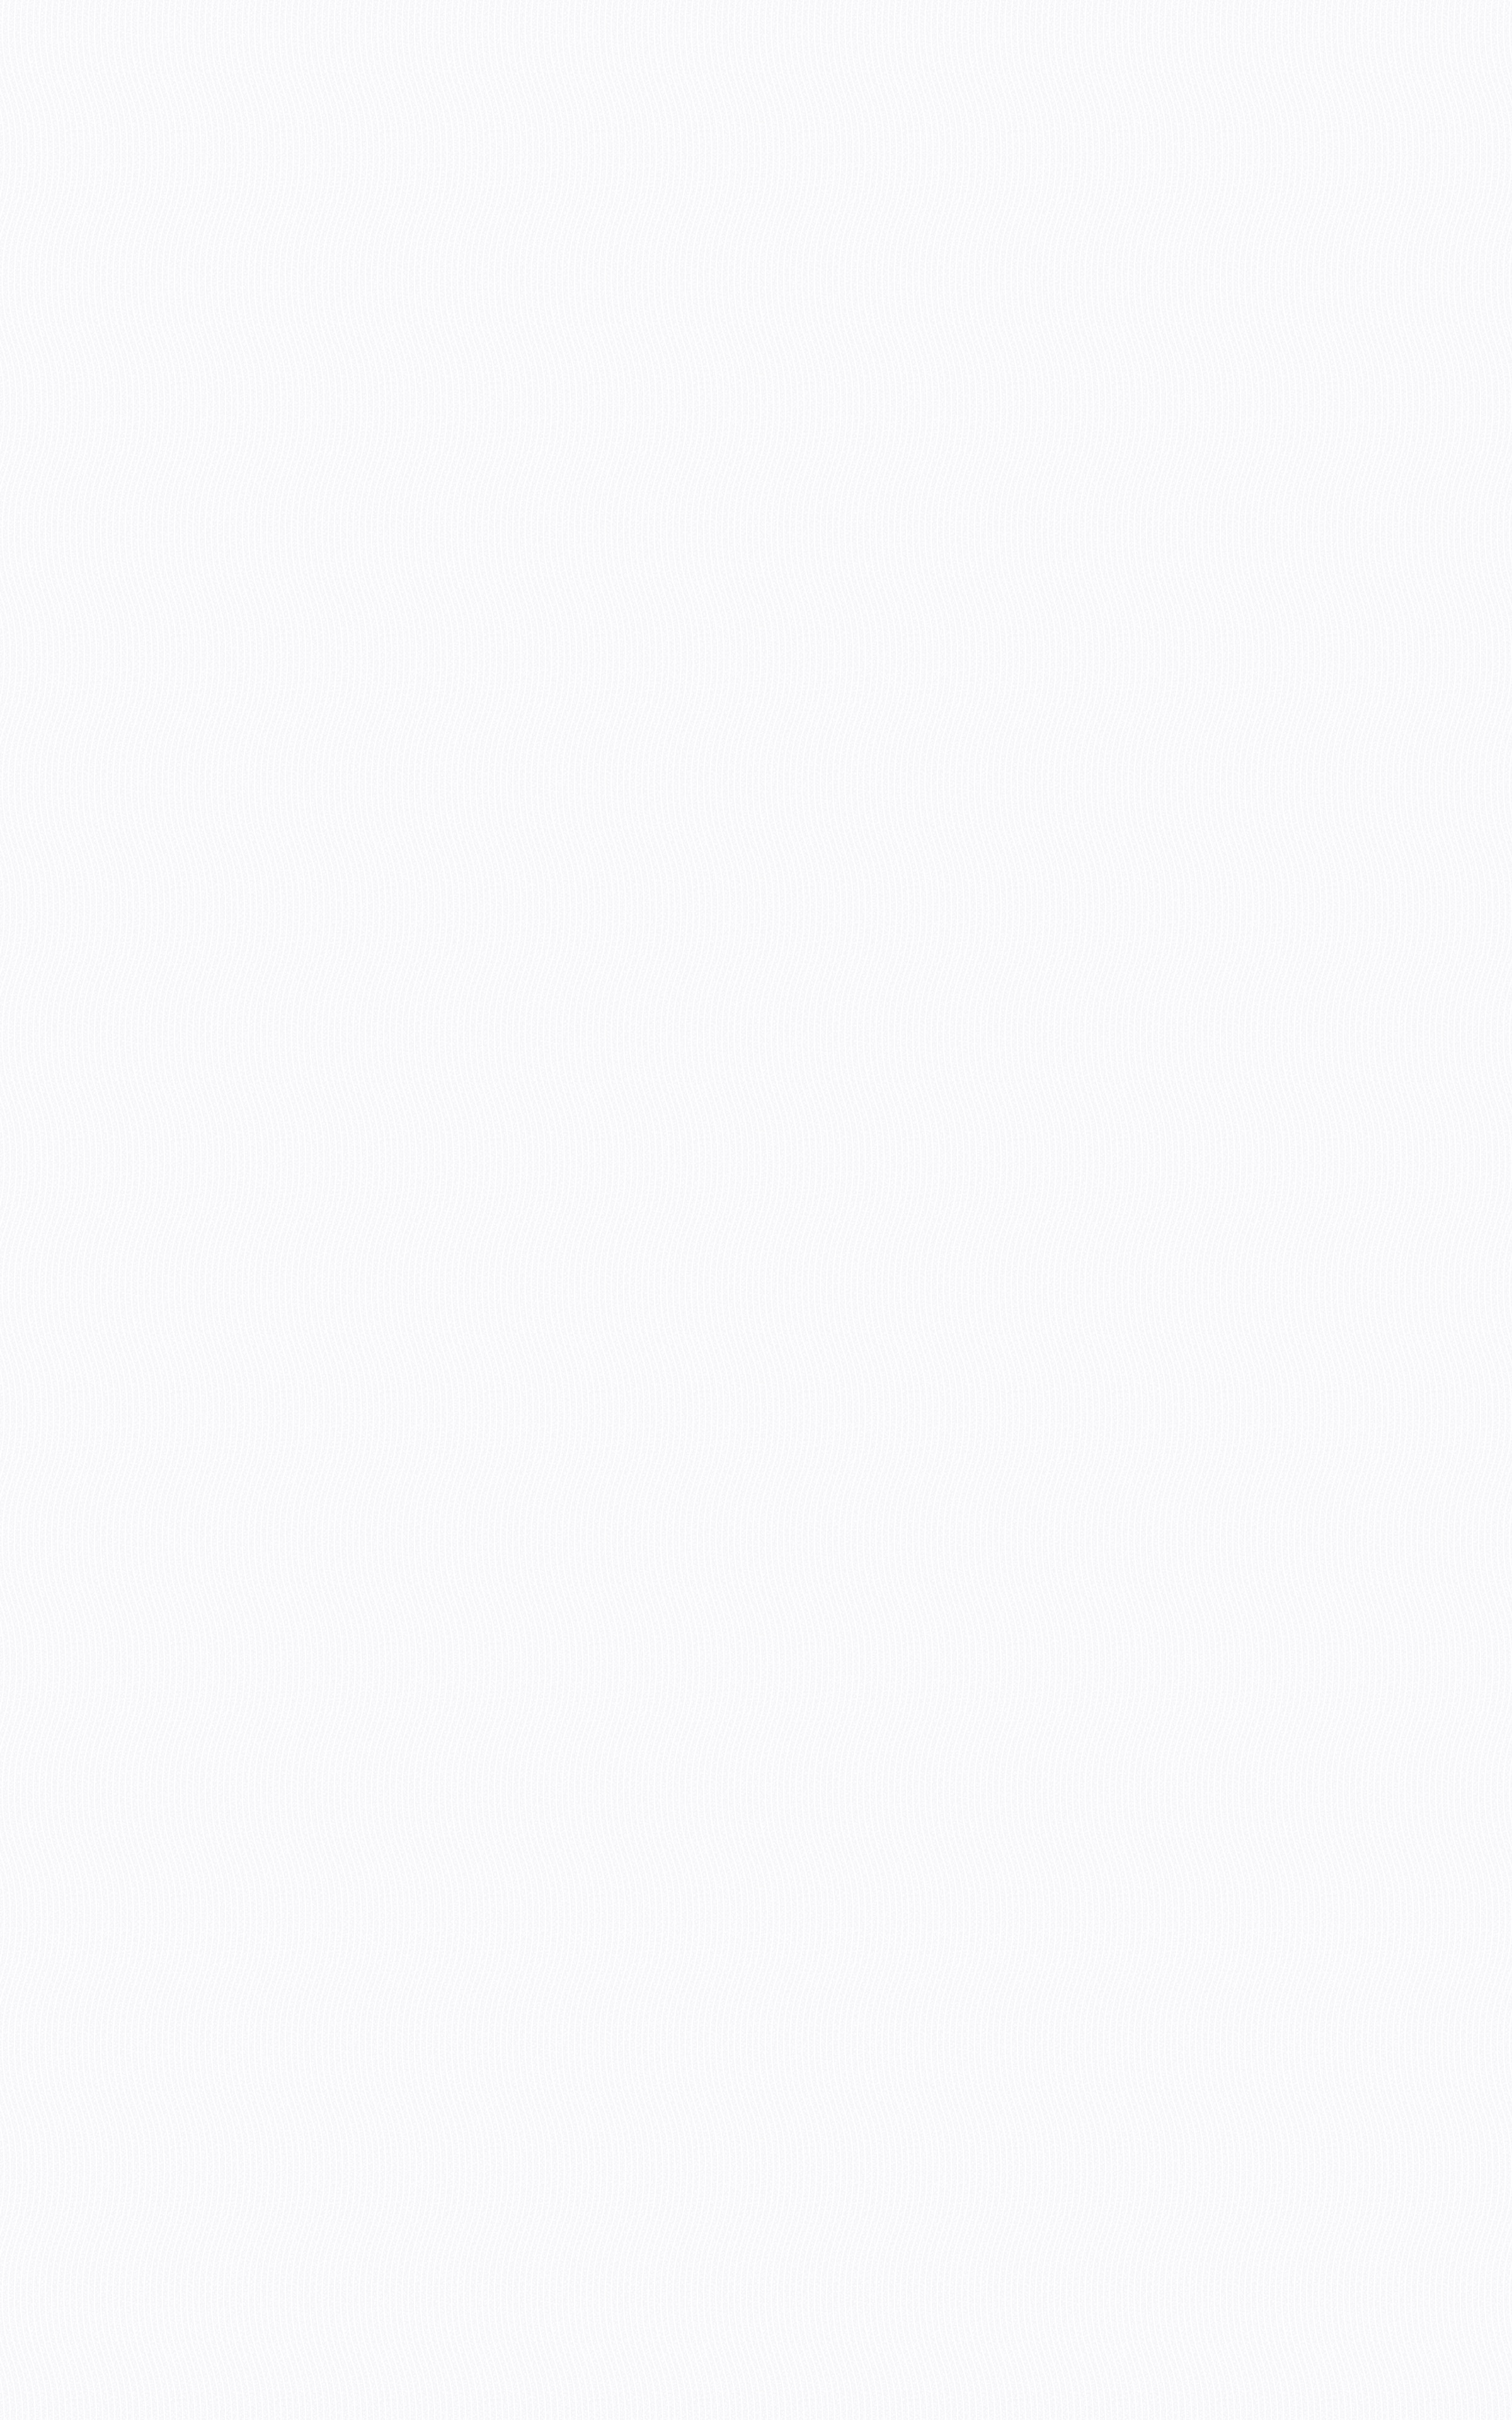
\includegraphics[width=\paperwidth, height=\paperheight, %
%%keepaspectratio]{images/background.jpg}%
%]{images/background.jpg}%
%\vfill
%}}}


\begin{document}
%\AddToShipoutPicture{\BackgroundPic}
\maketitle


\begin{abstract}
Loopring is an open protocol for building decentralized exchanges. Loopring operates as a public set of smart contracts responsible for trade and settlement, with an off-chain group of actors aggregating and communicating orders. The protocol is free, extensible, and serves as a standardized building block for decentralized applications (dApps) that incorporate exchange functionality. Important improvements over current decentralized exchange protocols are the ability for users' orders to be mix-and-matched with other orders, obviating the constraints of two-token trading pairs, drastically improving liquidity, and price improvement possibility. Loopring also employs a robust and unique solution to prevent front-running: the unfair attempt to submit transactions into a block quicker than the original solution provider. Loopring is blockchain agnostic, and deployable on any blockchain with smart contract functionality. At the time of writing, it's operable on Ethereum and QTUM, with NEO also under construction. Its interoperable standards ensure trustless, decentralized, and anonymous trading. 
\end{abstract}

\section{Introduction\label{sec:introduction}}

With the proliferation of blockchain-based assets, the need to exchange these assets amongst counterparties has significantly increased. As thousands of new tokens are introduced - including the tokenization of traditional assets - this need is magnified. Whether exchanging for speculative trading motivations, or converting to access networks via their native utility tokens, the ability to exchange one cryptoasset for another is foundational for the larger ecosystem.
 
As such, the trustless exchange of tokens (value) is a compelling use case for blockchain technology. Until now, however, crypto enthusiasts have largely settled for trading tokens on traditional centralized exchanges. The Loopring protocol is needed because, just as Bitcoin(1) dutifully pointed out that, in regards to peer-to-peer electronic cash, “the main benefits are lost if a trusted third party is still required to prevent double-spending”, so too are the main benefits of decentralized assets lost if they must pass through trusted, gated, centralized exchanges.

Trading decentralized tokens on centralized exchanges doesn't make sense from a philosophical perspective, as it fails to uphold the virtues these decentralized projects espouse. There are also numerous practical risks and limitations in using centralized exchanges which are described below. Decentralized exchanges (DEXs) have sought to address these issues, and in many cases have succeeded in alleviating security risks. However, there is still vast room for improvement in performance as DEX capability becomes important infrastructure for the new economy. Loopring hopes to provide critical tools for said infrastructure with its open protocol for building DEXs. 

\section{Current Exchange Landscape\label{sec:current_exchange_landscape}}

\subsection{Inadequacies of Centralized Exchanges}
The three primary risks of centralized exchanges are; 1) Lack of security, 2) Lack of transparency, and 3) Lack of liquidity.

\subsubsection{Lack of Security}
Security risks arise from the fact that users must typically surrender control of their private keys (funds) to one centralized entity. This exposes users to the possibility that centralized exchanges fall prey to malicious hackers. The security and hacking risks facing all centralized exchanges are well known(2), yet are often accepted as ‘table stakes' for token trading. Centralized exchanges, such as Coinbase and Bittrex, continue to be honeypots for hackers to attack, as their servers control millions of dollars of users' funds. Exchange developers can also make honest, accidental errors with your funds. You are simply not in control of your own tokens when they are deposited at a centralized exchange.

\subsubsection{Lack of Transparency}
Beyond security hacks, a lack of transparency exposes users to the risk of dishonest exchanges acting unfairly. The distinction here is by the exchange operator's malintentions. 

Users are not truly trading their own assets on a centralized exchange, but rather, an IOU - a promissory note that the exchange will redeem your note for your original asset. When tokens are sent to the exchange's wallet, they take custody, and offer an IOU. All trades are then effectively between users' IOUs. To withdraw, you redeem your IOU with the exchange, and get back your tokens to your external wallet address. Throughout this process there is a lack of transparency, and the exchange can shutdown, freeze your account, go bankrupt, etc. It is also possible that they use your assets for other purposes while in custody (such as lending them out to third parties), which makes you susceptible along another attack vector. Lack of transparency can also cost you without total loss of funds, such as in higher trading fees, delays at peak demand, regulatory risk, and your orders being front ran.

\subsubsection{Lack of Liquidity}
From the point of view of exchange operators, fragmented liquidity inhibits entry by new exchanges because of two winner-takes-all scenarios. First, the exchange with the most number of trading pairs available wins, because users find it desirable to conduct all their trades on one exchange. Second, the exchange with the largest order book wins, because of favorable bid-ask spreads for each trading pair. This discourages competition from newcomers because it is difficult for them to build up initial liquidity. As a result, many legacy exchanges command a high market share despite user complaints and even major hacking incidents. It's worth noting that as centralized exchanges win market share, they make themselves an ever-larger hacking target. 

From the point of view of users, fragmented liquidity significantly reduces user experience. In a centralized exchange, users are only able to trade within the exchange's own liquidity pools, against its own order book, and between its supported token pairs. To trade Token A, for Token B, you must go to an exchange that supports both tokens or register at different exchanges, disclosing personal information. You often need to execute preliminary or intermediate trades, usually against BTC or ETH, absorbing bid-ask spreads in the process. Finally, the order books may not be deep enough to complete your trade without material slippage.

The result is disconnected silos of liquidity and a fragmented ecosystem that resembles the legacy financial system, with significant trading volume centralized on few exchanges. The global liquidity promises of blockchains hold no merit within centralized exchanges.

\subsection{Inadequacies of Decentralized Exchanges}
Decentralized exchanges, such as KyberNetwork or EtherDelta, differ from centralized exchanges in that users maintain control of their assets (private keys) by performing trades directly on the underlying blockchain. By leveraging the trustless technology of cryptocurrencies themselves, they successfully mitigate many of the above mentioned risks surrounding security. However, problems persist in regards to performance and structural limitations. 

Liquidity often remains an issue as users must search for counterparties across disparate silos and standards. Fragmented liquidity effects are present if users don't employ consistent standards to interoperate, and if orders are not shared/propagated across a wide network. 

Furthermore, since trades are performed on chain, DEXs often inherit the limitations of the underlying blockchain, namely: scalability, delays in execution (mining), and costly modifications to orders. Thus, blockchain order books do not scale well, as executing code on the blockchain incurs a cost (gas), making multiple order-cancel cadences prohibitively expensive. 

Finally, because blockchain order books are public, the transaction to place an order is visible by miners as it awaits being mined into the next block, and placed into an order book. This delay exposes the user to the risk of being front run and having the price move against him.

\subsection{Hybrid Solutions}
For the above reasons, purely blockchain-based exchanges have limitations that make them uncompetitive with centralized exchanges. There is a tradeoff between on-chain inherent trustlessness, and centralized exchange speed and order flexibility. Protocols such as Loopring and 0x extend a solution of on-chain settlement with off-chain order relay. These solutions revolve around open smart contracts, but navigate scalability limitations by performing several functions off-chain, and giving nodes flexibility in fulfilling critical roles for the network. While Loopring admires protocols such as 0x, as we demonstrate throughout the paper, we propose meaningful differences in our approach to a hybrid solution.


\section{Loopring Protocol\label{sec:loopring_protocol}}
Loopring is not a DEX, but a protocol for building DEXs on multiple blockchains. We disassemble the component parts of a traditional exchange and offer a set of public smart contracts and decentralized actors in its place. The roles in the network include wallets, relays, liquidity-sharing consortium blockchains, order book browsers, ring-miners, and asset tokenization services. Before defining each, we should first understand what a Loopring compliant order looks like. 

\subsection{Order Ring}
Loopring orders are expressed in what we call a Unidirectional Order Model (UDOM (2)). UDOM expresses orders as token exchange requests - amountS/amountB - instead of bids and asks. Since every order is just an exchange rate between two tokens, a powerful feature of the protocol is the mixing and matching of multiple orders in circular trade. By using up to 10 orders instead of a single trading pair, there is a dramatic increase in liquidity and potential for price improvement. 

Each order's token to sell is another order's token to buy. It creates a loop that allows each order to exchange their desired tokens without requiring an opposing order for its pair. Traditional order pair trades can, of course, still be executed, in what is essentially a special case of an Order Ring. 


\begin{definition}[Order Ring] Let $C_{0}$, $C_{1}$, $\cdots$, $C_{n-1}$ be $n$ different kinds of token, $O_{0\rightarrow 1}$, $\cdots$, $O_{i\rightarrow i\oplus 1}$, $\cdots$, $O_{n-1 \rightarrow 0}$ be $n$ orders. Those orders can form a ring for trading:
$$O_{0\rightarrow 1} \rightarrow \cdots \rightarrow O_{i\rightarrow i\oplus 1} \rightarrow \cdots \rightarrow O_{n-1\rightarrow 0} \text{, }$$
where $n$ is the length of the ring, and $i\oplus 1 \equiv i+1 \mod n$.
\end{definition}

An order ring is valid when all component transactions can be executed at an exchange rate equal to or better than the original rate specified by the user. To verify ring validity, Loopring protocol smart contract (protocol) must receive Order Rings from miners where the product of the original exchange rates of all orders is equal to or greater than 1. (further calculations in section 4).

Every order has two basic elements: two assets offered for trading and an exchange rate. The price is the exchange rate with one of the assets fixed as parameter. Let assume Alice and Bob want to trade their tokens A and B. Alice has 15 tokens A and she wants 4 tokens B for them; Bob has 10 tokens B  and he wants 30 tokens A for them.

Who is buying and who is selling? This depends only on the asset we fix to give price quotations. If token A is the reference, then Alice is buying tokens B for ${15 \over 4} = 3.75$ XTA, while Bob is selling 10 tokens B for ${30 \over 10} = 3.00$ XTA. In the case of fixing token B as reference we say that Alice is selling 15 tokens A for ${4\over 15}=0.26666667$ XTB and Bob is buying 10 tokens A for ${10 \over 30}=0.33333334$ XTB. Hence, who's the buyer or seller is purely arbitrary.

In the first situation Alice is willing to pay a higher price than the price Bob is selling his tokens for, in the second situation Bob is willing to pay a higher price than the price Alice is selling her tokens for. It is clear that a trade is possible whenever the buyer is willing to pay an equal or higher price than the selling price, no matter how we fix the prices. If we recall our basic arithmetic we learned in school we can verify easily that:

\begin{equation}
{{15\over 4} \over {30\over 10}} = {3.75 \over 3.00}	= {0.33333334 \over 0.26666667} = {{10 \over 30} \over {4 \over 15}} = {15 \over 4} \cdot {10 \over 30} = {150 \over 120} = 1.25 > 1
\end{equation}

In this article, we reference this as the Uni-Directional Order Model, or UDOM for short. See \ref{anatomy} for more details about Loopring's orders.


\section{Ecosystem Participants}
The following ecosystem participants jointly provide all functionalities a centralized exchange has to offer. 

\begin{itemize}

\item \textbf{Wallets}: A common wallet service or interface that gives you access to your tokens and a way to send orders to the Loopring network. Wallets will be incentivized to produce orders by sharing fees (see section 5.1).

\item \textbf{Relays / Ring Miners}: Relays are nodes that form a decentralized network for order propagation. They maintain public order books and trade history and broadcast new orders to other relays via any arbitrary off-chain medium. Ring-mining is a feature of relays. It is computational heavy and is done completely off-chain. Ring-mining produces Order Rings: rings of between 2 and 10 tokens created by stitching together disparate orders. Relays are free in how they choose to communicate with one another (or not). 

\item \textbf{Consortium Liquidity Sharing Blockchain}: TODO(daniel)

\item \textbf{Loopring Protocol Smart Contracts}: A set of public and free smart contracts that checks Order Rings received from miners, does token transfers on behalf of users, incentivizes miners/wallets, and emits events. Relays/order browsers listen to these events to keep their order books and trade history up to date.

\item \textbf{Asset Tokenization Services}: A bridge between assets that cannot be directly traded on Loopring. They are centralized services run by trustworthy companies or organizations. A user could deposit his assets (real, fiat or tokens from other chains) and get tokens issued. By returning these tokens the user gets back his deposit. Loopring is not a cross-chain exchange protocol, but Asset Tokenization Services make it possible to trade Ethereum ERC20 tokens with physical assets as well as assets on other blockchains. 

\end{itemize}


\section{Exchange Process}
\begin{enumerate} 

\item \textbf{Order Initiation \& ERC20 Authorization}: A user wants to exchange X amount of TokenA for Y amount of TokenB. The current rate and order book for this pair can be found on multiple sources provided by relays or other interfaces hooked up to the network, such as order book browsers (4). The user places an order through a wallet interface. An amount of LRx can be added to the order as a fee for miners; higher LRx fee means a better chance to be processed earlier by miners. The wallet authorizes the LSC to handle X amount of TokenA the user wants to sell, but does not lock the user's tokens, who remains free to move them while the order is being processed.

\item \textbf{Send order to the network}: Once the authorization is made, the order's data is signed with the private key of the sender. Then, the wallet sends the order along with its signature to one or more nodes (relays) in the network.
\item \textbf{Relay broadcast}: On the reception of the order, relays update their public order book and broadcast the order to other relays/ring miners. The protocol doesn't require order books to be built in a certain way, for example, first-come-first-serve. Instead, relays have the power to make their own design decisions to build their own order books.
\item \textbf{Ring-mining (order matching)}: Ring Miners receive the order and add it to their order book. Each miner tries to fill it fully or partially at the given exchange rate or better by ring-matching it with multiple other orders. Ring-matching is the main reason why the protocol is able to provide high liquidity over any pair. If the executed rate is better than what the user asked for, the savings (margin) are shared amongst all orders in the ring. As a reward (fee), the miner can choose between claiming the Margin Split and giving back the LRx to the user, or just keeping the LRx fee.
\item \textbf{Verification \& Settlement}: The ring is received by the Loopring Smart Contract. It makes multiple checks to verify the miner's supplied data and determines if the ring can be settled fully or partially (depending on the fill rate of orders in the ring and the tokens in the users' wallets). If all checks are successful, the contract automatically makes the token transfers to the users and pays the miner's fees at the same time. If the sender's balance as determined by the LSC are insufficient, it will be considered scaled-down. A scaled-down order is not the same as a cancelled order: a scaled-down order will automatically scale up to its original size if sufficient funds are deposited to its address, while cancellation is a one way manual operation and can't be reversed.

\end{enumerate}

\section{Business Model Flexibility}
It's important to note that Loopring's open standard allows participants significant flexibility in how they conduct ‘business'. Actors with novel business models are free to implement them and provide value for their users, earning LRx fees on volume in the process.
\subsection{Order Book}
Relays can design their order books in any number of ways to display and match users' trades. A first implementation of our own order book follows an OTC model, where limit orders are ‘ranked' or positioned based on price alone. Timestamps of orders, in other words, have no bearing on the order book. However, a relay is free to design their order book in such a way as to emulate a typical centralized exchange's matching engine, where orders are ranked by price, but with a timestamp respecting filter as well. If a relay was inclined to offer this type of order book, they can own/integrate with a wallet, and have those wallet orders sent solely to the single relay, who would then be able to match orders based on time. Any such configuration is possible. 

\subsection{Liquidity Sharing}
Relays are similarly free to design how they share liquidity and orders with one another. Our consortium blockchain is but one solution to accomplish this, and the ecosystem is free to network and communicate as they wish. Besides joining a consortium blockchain, they can build and manage their own, creating rules/incentives as they see fit. Relays can also work solo, as seen in the time-sensitive wallet implementation above. Of course, there are clear advantages in communicating with other relays in pursuit of network effects, however, different business models could merit peculiar sharing designs. 



\section{Protocol Specification}

\subsection{Anatomy of an Order\label{anatomy}}
An order is a pack of data that describes the intent of the user's trade. A Loopring order is defined using the Uni-Directional Order Model, or UDOM, as follows:

\begin{verbatim}
  message Order {
    address protocol;
    address owner;
    address tokenS;
    address tokenB;
    uint256 amountS;
    uint256 amountB;
    unit256 lrcFee
    unit256 validSince;             // Seconds since epoch
    unit256 validUntil;             // Seconds since epoch
    uint8   marginSplitPercentage;  // In the rage of [1-100]
    bool    buyNoMoreThanAmountB;
    uint256 walletId;
    address authAddr; // Dual-Authoring address
    uint8   v;        // Part of the signature
    bytes32 r;        // Part of the signature
    bytes32 s;        // Part of the signature
    string  _authKey; // Dual-Authoring private key,
                      // it is not used for calculating order's hash.
  }
\end{verbatim}
To ensure the origin of the order, it is signed against the hash of its parameters, excluding $\_authAddr$, with the user's private key. The $\_authAddr$ parameter is used for signing  order rings that this order is part of, which prevents front-running. Please reference \ref{dual_authoring} for more details. The signature is represented by the $v$, $r$, and $s$ fields, and is sent alongside the order parameters over the network. This guarantees the order stays immutable during its whole lifetime. Even though the order never changes, the protocol can still compute its current state based on the balance of its address along with other variables.


UDOM doesn't include a price (which must be a floating-point number by nature), but, instead uses the term $rate$, which is expressed as $amountS \over amountB$. The rate is not a floating-point number but an expression that will only be evaluated with other unsigned integers on demand, to keep all intermediate results as unsigned integers and increase calculation accuracy. 

When a miner ring-matches orders, it's possible that a better rate will be executable, allowing you to get more $tokenB$ than the $amountB$ you specified. However, if $buyNoMoreThanAmountB$ is set to $true$, the protocol ensures you receive exactly $amountB$ of $tokenB$. Thus, UDOM's $buyNoMoreThanTokenB$ parameter determines when an order is considered completely filled. $buyNoMoreThanTokenB$ applies a cap on either $amountS$ or $amountB$, and allows users to express more granular trade intentions than traditional buy/sell orders. 

If we use

\begin{equation}
	Order(amountS, tokenS, amountB, tokenB, buyNoMoreThanTokenB)
\end{equation}

to represent a order in a simplified form, then for ETH/USD markets on a traditional exchange, traditional buy-sell modeling can express the 1st and the 3rd order below, but not the other two:

\begin{enumerate}
	\item User wants to sell 10 ETH at price 300 USD/ETH. This order can expressed as $Order(10, ETH, 3000, USD, false)$.
	\item User wants to sell ETH at price 300 USD/ETH to get 3000 USD. This order can expressed as $Order(10, ETH, 3000, USD, true)$.
	\item User wants to buy 10 ETH at price 300 USD/ETH, This order can expressed as $Order(3000, USD, 10, ETH, true)$.
	\item User wants to spend 3000 USD to buy as many ETH as possible at price 300 USD/ETH, This order can expressed as $Order(3000, USD, 10, ETH, false)$.
\end{enumerate}





\subsection{Ring Verification}

LSC does not perform exchange rate or amount calculations, but must receive and verify what the miner supplied for these values. This is done by miners for two main reasons: solidity does not have support for floating point maths, especially pow(x, 1/n), and it is desirable for the computation to be made off-chain to save gas.

\subsubsection{Sub-Loop Checking}
This step prevents arbitrageurs from unfairly realizing all the margin in a ring by implementing new orders within it. Essentially, once a valid ring is found by a miner, it could be tempted to add other orders to the ring to fully absorb the users' margin (rate discounts). This is zero-risk, zero-value add to the network, and is considered unfair conduct by the miner. To prevent this, Loopring requires that a valid loop cannot contain a sub-loop. To check this, LSC ensure a token cannot be in a buy or sell position twice. In the above diagram we can see that ARK is a sell token twice, and a buy token twice, which would be disallowed. 

\subsubsection{Fill Rate Checking}
The exchange rate calculations in the ring are made by miners for reasons stated above. It is the LSC that must verify they're correct. First, it verifies that the buy rate the miner can execute for each order is at least equal to or less than the original buy rate set by the user. This ensures the user gets at least the exchange rate they asked for or better on the transaction. Once the exchange rates are confirmed, LSC makes sure that all the margins (discounts) are the same percentage for every order, to ensure fairness.

According to Loopring protocol, each order in the ring would share the same rate (price) discount. For instance, if the discounted rate is $\gamma$, then the price for each order will be:
$r_{0\rightarrow 1} \cdot (1-\gamma)$, $r_{1\rightarrow 2} \cdot (1-\gamma)$, $r_{2 \rightarrow 0} \cdot (1-\gamma)$, and satisfied: 
\begin{equation}
r_{0\rightarrow 1} \cdot (1-\gamma)\cdot r_{1\rightarrow 2} \cdot (1-\gamma) \cdot r_{2 \rightarrow 0} \cdot (1-\gamma) = 1
\end{equation}
We can find out: 
\begin{equation*}
\gamma = 1- \frac{1}{\sqrt[3]{r_{0\rightarrow 1} \cdot r_{1\rightarrow 2} \cdot r_{2\rightarrow 0}}}\text{.}
\end{equation*}
In the other circumstance, if transaction cross $n$ orders, the \texttt{discount} is: 
\begin{equation*}
\gamma = 1- \frac{1}{\sqrt[n]{\prod_{i=0}^{n-1} r^i}} \text{,}
\end{equation*}
where $r^i$ is the order turnover rate of $i$-th order. Obviously, only when the discount rate is $\gamma \ge 0$, these orders can be filled; and the $i$-th order's $O^i$ actual exchange rate $\hat{r^i} = r^i \cdot (1-\gamma)$, $\hat{r^i}\le r^i$.

\subsubsection{Fill Tracking \& Cancellation}
A user can partially or fully cancel an order by sending a special transaction to the LSC, containing the details about the order and the amounts to cancel. The LSC takes that into account, stores the amounts to cancel, and emits an OrderCancelled event to the network. The LSC keeps track of fill and cancellation amounts by storing their values using the order's hash as an identifier. This data is publicly accessible and OrderCancelled / OrderFilled events are emitted when it changes. Tracking these values is critical for the LSC during the ring settlement step.


\subsubsection{Order Scaling}
Orders are scaled according to the history of filled and cancelled amounts and the current balance of the senders' accounts. The process finds the order with the smallest amount to be filled according to the above characteristics and uses it as a reference for scaling all transactions in the ring.


Finding the lowest value order can help to figure out the fill volume for each order. For instance, if the $i$-th order is the lowest value order, then the number of tokens sold from each order $\hat{s}$ and number of tokens purchased $\hat{b}$ from each order can be calculated as:

\[
\begin{split}
&\hat{s}^{i}=\overline{s}_i\text{, } \hat{b}^{i}=\hat{s}^{i}/ \hat{r}^i\text{, }\text{;}\\
&\hat{s}^{i\oplus 1}=\hat{b}^i\text{, } \hat{b}^{i\oplus 1}=\hat{s}^{i\oplus 1}/ \hat{r}^{i\oplus 1}\text{;}\\
&\hat{s}^{i\oplus 2}=\hat{b}^{i\oplus 1}\text{, } \hat{b}^{i\oplus 2}=\hat{s}^{i\oplus 2}/ \hat{r}^{i\oplus 2}\text{;}\\
& ...
%\text{.}
\end{split}
\]
where $\overline{s}_i$ is the the balance left after orders are partially filled.

During implementation we can safely assume any order in the ring to have the lowest value, then iterate through the ring at most twice to calculate each orders' fill volume. 

Example: If the smallest amount to be filled compared to the original order is 5\%, all the transactions in the ring are scaled down to 5\%. Once the transactions are completed, the order that was considered to have the smallest amount remaining to be filled should be completely filled.

\subsection{Ring Settlement}

If the Order Ring fulfills all the previous checks, the ring can be closed, and transactions can be made. This means that all the $n$ orders $O$ form a closed ring of orders, connected as in the figure below:

[TODO: DIAGRAM]

To make the transactions, the LSC uses the $TokenTransferDelegate$ smart contract. The introduction of such a delegate makes upgrading the protocol smart contract easier as all orders only need to authorize this delegate instead of different versions of the protocol.

For each order in the ring, a payment of $tokenS$ is made to the following order. Then the miner's fee is paid depending on the fee model chosen by the miner. An $OrderFilled$ event is then emitted. Finally, once all the transaction are made, a $RingMined$ event is emitted.

\subsubsection{Emitted Events}

The protocol emits events that allow relays, order browsers, and other actors to receive order book updates as efficiently as possible. The emitted events are:

\begin{itemize}
	\item \textbf{OrderCancelled}: a specific order has been cancelled.
	\item \textbf{OrdersCancelled}: all orders of a trading pair for an owning address have been cancelled.
	\item \textbf{AllOrdersCancelled}: all orders of all trading pairs for an owning address have been cancelled.	
	\item \textbf{RingMined}: A ring has been settled successfully. This event contains data related to each inner-ring token transfer.
\end{itemize}


\section{LRx Token}
LRx is our generalized token notation. LRC is the Loopring token on Ethereum, LRQ on QTUM, and LRN on NEO. More LRx will be introduced in future as Loopring is deployed on other public blockchains.

\subsection{Fee Model} 
When a user creates an order, they specify an amount of LRx to be paid to the miner as a fee, in conjunction with a percentage of the margin made on the order that the miner can claim. This is called the margin split. The decision of which one to choose is left to the miner.

A representation of the margin split:

[TODO: daniel wang]

If the margin on the ring is too small, a miner will choose the LRx fee. On the contrary, if the margin is substantial enough for the resulting margin split to be worth more than the LRx fee, they will choose the margin split. There is another proviso, however: when the miner chooses the margin split, they must pay the user (order creator) a fee, which is equal to the LRx the user would have paid to the miner as a fee. This increases the threshold of where the miner will choose the margin split to twice the LRx fee of the order, increasing the propensity of the LRx fee choice. This allows miners to get a constant income on low margin rings with for the tradeoff of getting less income on higher margin rings. Our fee model is based on the expectation that as the market grows and matures, there will be fewer high margin rings, thus necessitating LRx fees as incentive.
We end up with the following graph:

[TODO: daniel wang]

where $f$ is the LRx fee, $x$ is the margin split, $y$ is the miner's income.

If $f$ is the LRx fee and $x$ the margin split, then the miner's income $y$ is $y=max(f, x-f)$ and we get the blue line; if the LRx fee for the order is $0$, the equation is $y=max(0, x - 0)$ that simplifies to $y=x$ and we get the orange line.

The consequences are:  
\begin{enumerate}
	\item If the margin split is 0, the miners will choose the flat LRx fee and are still incentivized. 
	\item If the LRx fee is 0, the orange line results and the income is based on a general linear model.
	\item When the margin split income > 2*(LRx fee), the miner chooses the margin split.
\end{enumerate}

It should be noted that if the LRx fee is non-zero, no matter which option the miner chooses, there will always be a transfer of LRx between the miner and the order's sender. Either the miner earns the LRx fee, or pays the LRx fee back to the sender to take the margin split.

Ring miners will share a certain percentage of fees with wallets. When a user places an order through a wallet and it is filled, the wallet is rewarded with a portion of the fees or margin split. Wallets represent a primary target for protocol integration as they have the user base, but little source of income. 

\subsection{Decentralized Governance}
LRx tokens are used to align the financial incentives of the various participants in the network. Such alignment is necessary for broad adoption of the protocol, whose success rests largely on improving liquidity in a robust decentralized ecosystem.

LRx tokens will be used to effectuate protocol updates through decentralized governance. Smart contract upgrades will be voted on by token holders to dissuade rogue forks from potentially siphoning off liquidity through incompatibility. Upgradeability is crucial to the protocol's success as it must adapt to market demands, and the changing underlying blockchains.

\section{Fraud and Attack Protections}

\subsection{Dual-Authoring: Front-running Prevention}

In decentralized exchanges, front-running is when someone tries to copy another node's ring solution, and have it mined before the original transaction that is in the pending transaction pool (mempool). This can be achieved by specifying a higher transaction fee (gas price). The major scheme of front-running in Loopring (and any protocol for order-matching) are order-filch: when a front-runner steals one or more orders from a pending ring settlement transaction; and Ring-filch: when a front-runner steals the entire ring from the pending transaction.

When a submitRing transaction is not confirmed and still in the pending transaction pool, anyone can easily spot such a transaction and replace $miner\_address$ with their own address (the filcher\_address) , then they can re-sign the payload with filcher\_address to replace the ring's signature. The fincher can set a higher gas price and submit a new transaction hoping block miners will pick his new transaction into the next block instead of the original submitRing transaction.
Previous solutions to this problem had important downsides (v1.1): it requires more transactions and thus cost miners more gas; and it takes at least twice the blocks to settle a ring.  Our new solution involves the mechanism of setting up two levels of authorization for orders - one for settlement, and one for mining.
How it works:

\begin{enumerate}

	\item For each order, the wallet software will generate a random public- key/private-key pair, and put the key pair into the order's JSON snippet. (An alternative is to use the address derived from the public-key instead of the public-key itself to reduce byte size. We use $authAddr$ to represent such an address, and $\_authKey$ to represent $authAddr$'s matching private-key).

	\item All fields in the order except $\_authKey$ is signed using the $owner$ address's private-key (not $\_authKey$) as shown in the image below.

	\item The wallet will send the order, together with the $\_authKey$ to miners (relays) for matching.The miner will verify that $\_authKey$ and $authAddr$ are correctly paired and the order's signature is valid with respect to owner\_address.

	\item When a ring is identified, the miner will use each order's $\_authKey$ to sign the ring's hash, $miner\_address$, and all the mining parameters. In the example below, the ring contains 3 orders, therefore there will be 3 signatures by the 3 $\_authKey$s. We call these signatures the $auth\_signature$s. The miner also needs to sign the ring's hash together with all mining parameters using $miner\_address$'s private-key.

	\item The miner calls the submitRing function with all the parameters, as well as the 3 extra $auth\_signature$s. Notice that$\_authKey$s are NOT part of the on-chain transaction and thus remain unknown to people other than the relay itself, as shown in the image below.

	\item The Loopring Protocol will now verify each $auth\_signature$ against the corresponding $authAddr$ of each order, and reject the ring if any $auth\_signature$ is invalid.
 
\end{enumerate}
[TODO: daniel wang]


The result it that now:

\begin{itemize}

	\item  The order’s signature (by the private-key of the $owner\_address$) guarantees the order cannot be modified, including the $authAddr$.
	\item  The miner’s signature (by the private-key of the $miner\_address$) guarantees nobody can use his identity to mine a ring.
	\item  The $auth\_signature$s guarantees the entire ring cannot be modified, including $miner\_address$. And since ring-filchers do not have access to $\_authKey$s, they cannot re-generate a new set of $auth\_signature$s thus are unable to generate a filch transaction.

\end{itemize}

Dual Authoring prevents ring-filch and order-filch while still ensuring the settlement of rings can be done in one single transaction. In addition, Dual Authoring opens doors for relays to share orders in two ways: non-matchable sharing and matchable sharing. Loopring operates an OTC model, meaning that orders’ timestamps are totally ignored. This implies that front-running a trade has no impact on the actual price of that trade .  Loopring only supports limit-price orders.

\section{Other Attacks}

\subsection{Denial of Service}
Loopring allows nodes (relayers) to selectively handle orders by setting their own criteria - which they may hide or reveal. By empowering relayers to dictate how they manage orders, we do not see denial of service as a form of unethical behaviour.

\subsection{Sybil Attack}
A user could send a large amount of tiny orders to attack the Loopring nodes. However, since we allow nodes to reject orders based on their own criteria, most of these orders will be rejected because they do not yield satisfying profit when matched. Thus, a massive tiny order attack is not feasible.

\subsection{Insufficient Balance}
Malicious users may sign and spread out orders whose value inside the order is non-zero but whose address actually has zero balance. Nodes could monitor and notice that some orders actual balance is zero, update these orders states accordingly and then discard them.
Nodes have to spend time to update the status of an order, but can also choose to minimize the effort by, for example, blacklisting addresses and drop related orders.


\section{Summary}
Money, as an intermediate commodity, is used to facilitate barter exchange and solve the double coincidence of wants problem (6). Similarly, Loopring protocol aims to dispense of our dependencies on coincidence of wants in trading pairs. With ring matching, double coincidence of wants is no longer required before a trade could be consummated. This is profound for how society and capital markets transfer value with tokens, traditional assets, and beyond.

\begin{itemize}
	\item Off-chain order management and on-chain settlement = no sacrifice in performance for security.
Network is maintained by a self-motivated group of relays who have flexibility in running their order books.
	\item Greater liquidity due to more counterparties available through order sharing, and increasing probability that any counterparty can be a useful trading partner due to multi-party trades.
	\item Orders can be propagated through arbitrary communication mediums, and liquidity siloes can be connected.
	\item Free, public smart contracts enable any dApp to build or interact with our protocol.
	\item Standardization among operators allows for network effects, deeper liquidity and an improved end user experience.
	\item Reduced barriers to entry for market makers mean lower costs for nodes joining the network and end users.
	\item Anonymous trading directly from users’ wallets.
\end{itemize}

\section{Acknowledgements}
We would like to express our gratitude to our mentors, advisers and to the many people in the community that have been so welcoming and generous with their knowledge. In particular, we would like to thank Shuo Bai (from ChinaLedger); Professor Haibin Kan; Alex Cheng, Hongfei Da; Yin Cao; Xiaochuan Wu; Zhen Wang, Wei Yu, Nian Duan, Jun Xiao, Jiang Qian, Jiangxu Xiang, Yipeng Guo, Dahai Li, Kelvin Long, Huaxia Xia, Jun Ma, and Encephalo Path for reviewing and providing feedback on this project. We also welcome more feedback from the community.

\bibliography{whitepaper}
\bibliographystyle{unsrt}

\section{===========}






















\section{Market and Industry\label{sec: existingworks}}

Today, decentralized exchange protocols built on blockchain technology already exist. Examples include Ripple, BitShares, Openledger, Bancor, and 0x.

Ripple\cite{schwartz2014ripple} is a real-time gross settlement system, currency exchange, and remittance network operated by Ripple (the company). The Ripple Transaction Protocol (RTXP) or Ripple protocol, it is built upon a distributed open source Internet protocol also known as the consensus ledger. Ripple's solution is built around an open, neutral protocol (Interledger Protocol or ILP\cite{thomas2015protocol}) that powers payments across different ledgers and networks globally. It offers a cryptographically secure end-to-end payment flow with transaction immutability and information redundancy. Architected to fit within a bank's existing infrastructure, Ripple is designed to comply with risk, privacy, and compliance requirements.

BitShares\cite{schuhbitshares}\cite{schuh2015bitshares} is an industrial grade financial blockchain smart contract platform. The BitShares decentralized exchange - also known as "The DEX" is a next-generation cryptocurrency trading platform. The DEX is inherently decentralized, enabling one to trade the BitShares core token (BTS) and a range of trustless price-stable, market-pegged assets, such as bitUSD, bitCNY, bitBTC, bitGold, and others. These assets can all be traded with zero counter-party risk, putting the user in total control of their funds. However, the Bitshares project has many limitations.

The OpenLedger Dex\cite{openledger} is a cryptocurrency exchange. It allows users to exchange Bitcoin into smartcoins and then withdraw the smartcoins and convert them into cash through PayPal, Ripple, or NanoCard. Additionally, Openledger relies greatly on the BitShares 2.0 platform and Graphene Toolkit's operation.

The Bancor\cite{bancor}\cite{hanson2012logarithmic} protocol enables built-in price discovery and a liquidity mechanism for tokens on smart contract blockchains. These "smart tokens" hold one or more other tokens in reserve and enable any party to instantly purchase or liquidate the smart token in exchange for any of its reserve tokens. This is done directly through the smart token's contract, at a continuously calculated price according to a formula which balances buy and sell volumes.

"0x"\cite{warren20170x} is a protocol that facilitates low friction peer-to-peer exchange of ERC20\cite{ERC20} tokens on the Ethereum blockchain. The protocol is intended to serve as an open standard and common building block driving interoperability among decentralized applications (dApps) that incorporate exchange functionality. Trades are executed by a system of Ethereum smart contracts that are publicly accessible, free to use and that any dApp can hook into. DApps built on top of the protocol can access public liquidity pools or create their own liquidity pool and charge transaction fees on the resulting volume. However, 0x protocol has limitations including  only being able to accept simple OTC orders, having an unclear competing mechanism among different exchanges, and lacking a protection mechanism for miners.

Taking in to account the advantages and limitations stated above, it is clear that centralized exchange still plays an important role in the cryptocurrency market at present. Nevertheless, Our team, inspired by both 0x protocol and payment channel, have conceived a new solution for a decentralized exchange protocol.


\section{Protocol Design\label{sec: protocol}}

\begin{center}
\begin{figurehere}
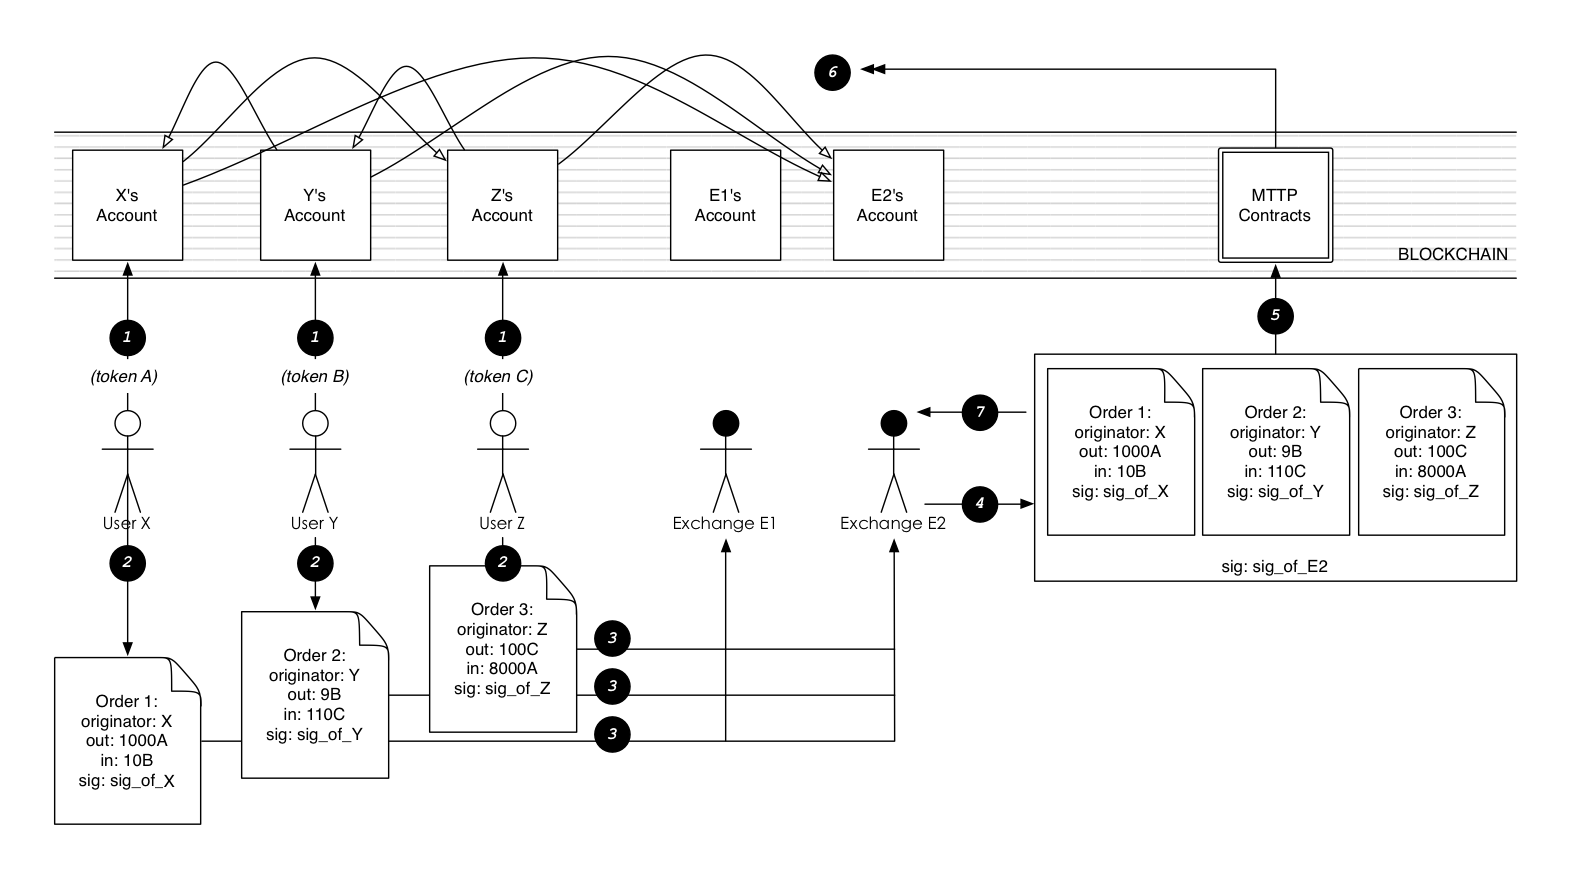
\includegraphics[height=8cm]{images/en_protocol.png}
\caption{Figure shows mix and match 3 orders}
\label{fig: Loopringrotocol}
\end{figurehere}
\end{center}

Figure 1 presents the general sequence of steps used for three separate transactions under Loopring:

\begin{enumerate}
 \item User X, Y, and Z authorize the Loopring smart contract to access their accounts for token trading. From the above figure, such a contract may transfer out 1000 A tokens from User X's account, transfer out 9 B tokens from User Y's account, and 100 C tokens from User Z's account;
 \item User X, Y, and Z place their own orders with signature using their private keys. Thus, all orders go into a medium and are ready to be exchanged - Order 1 is selling no more than 1000 A tokens and purchasing no less than 10 B tokens; if the order is partially matched,  then the exchange rate between tokens A to B should be no less than 1000/10=100.00 (number of tokens sold divided by number of tokens purchased). Furthermore, to illustrate other parameters involved in chapter 3.7;
 \item User X, Y, and Z continue to send their orders to one of the other multiple exchanges;
 \item After the exchange received all three separated orders, they will replace them into a corresponding order-book, while updating a new block and calculating each orders status to match the set order - creating a loop we delineate as a ring exchange or matching exchange. Once all the orders are confirmed and successfully mix-matched;
 \item Exchange will send out a signature to the given Loopring smart contract address;
 \item Loopring smart contract will verify quadruple signatures in order to verify three orders closing. If closing fails, the contract will be terminated (certain exchange gas cost exempt); otherwise, Loopring smart contract needs to calculate the proceeds and cost for each users, to complete the token exchange --- as illustrated in the figure below. During each step, Loopring smart contract will use Loopring Registration Contract to calculate all the fees and discount before closing. The system will also need to use Loopring Stats Contract to update the database.

\begin{center}
\begin{figurehere}
\includegraphics[height=5cm]{images/en-Loopring-example.png}
\caption{Loopring:Match-Ring Settlement}
\label{fig:Loopringprotocol}
\end{figurehere}
\end{center}
  
  
 \item Exchange begins receiving new block and new data from the chain in order to update the order-book to mix-match new and existing orders.
\end{enumerate}


\subsection{Definition of Symbol}

Symbols are defined as follows.
\[
\begin{split}
&C_{i}\text{: \ }\text{stands for the $i$-th token.}\\
&O_{i\rightarrow j}\text{: \ }\text{stands for an order selling token $C_{i}$ for token $C_{j}$ .}\\
&s_{i\rightarrow j}\text{: \ }\text{selling token upper limit in order $O_{i\rightarrow j}$.}\\
&b_{i\rightarrow j}\text{: \ }\text{buying token lower limit in order $O_{i\rightarrow j}$.}\\
&r_{i\rightarrow j}\text{: \ }\text{max exchange rate in order $O_{i\rightarrow j}$, which is $s_{i\rightarrow j} / b_{i\rightarrow j}$.}
\end{split}
\]


We underlined the symbols to place emphasis on their original numbers. For example $\overline{s}_{i\rightarrow j}$ and $\overline{b}_{i\rightarrow j}$ stands for the number of tokens from the original order.

\subsection{Rate Immutability\label{sec: consistrate}}

Loopring requires that the max-return exchange rate in an order remains immutable until the order is closed: 
$s_{i\rightarrow j} / b_{i\rightarrow j} = \overline{s}_{i\rightarrow j}/ \overline{b}_{i\rightarrow j}$. This guarantees that after an order is partially filled, the remaining order still satisfies the user's original intention.

\subsection{Order Reducibility\label{sec: reducibility}}


We can use token $C_j$ to connect two orders ( $O_{i\rightarrow j}$ and $O_{j\rightarrow k}$ ), to recognize it as one single order for selling token $Ci$ for buying token $C_k$. we use $O_{i\rightarrow j\rightarrow k}$ to represent this order. The resulting $O_{i\rightarrow k}$'s properties can be calculated as: 

\begin{equation}
s_{i\rightarrow j\rightarrow k}=min(b_{i\rightarrow j}, s_{j\rightarrow k}) \cdot r_{i\rightarrow j}
\end{equation}

\begin{equation}
b_{i\rightarrow j\rightarrow k}=min(b_{i\rightarrow j}, s_{j\rightarrow k}) / r_{j\rightarrow k}
\end{equation}

\begin{equation}
r_{i\rightarrow j\rightarrow k}= r_{i\rightarrow j}\cdot r_{j\rightarrow k}
\end{equation}


Here we introduce the concept of an order-chain. It contains two or more orders, each selling token order is the following  purchasing token order except the last one in the chain. Additionally, final purchasing token order should be different from the first orders selling token (otherwise it will become ring).

\[ s_{0\rightarrow ...\rightarrow n} =
 \begin{cases}
  s_{0\rightarrow 1}   & \quad \text{as } n \text{ = 1}\\
  min(b_{0\rightarrow ...\rightarrow n-1}, s_{n-1\rightarrow n}) \cdot r_{0\rightarrow ...\rightarrow n-1} & \quad \text{as\ } n \text{ $>$ 1}\\
 \end{cases}
\]

\[ b_{0\rightarrow ...\rightarrow n} =
 \begin{cases}
  b_{0\rightarrow 1}   & \quad \text{as } n \text{ = 1}\\
  min(b_{0\rightarrow ...\rightarrow n-1}, s_{n-1\rightarrow n}) / r_{n-1\rightarrow n} & \quad \text{as\ } n \text{ $>$ 1}\\
 \end{cases}
\]


\[ r_{0\rightarrow ...\rightarrow n} = \prod_{i=0}^{n-1}{r_{i\rightarrow i+1}}
\]


\subsection{Match-Ring}

Most, if not all, centralized exchanges match orders from the two sides of a trading pair. Loopring, however, detects a ring of orders that may involve multiple tokens/currencies. With one order Match-Ring, multiple orders can be filled instantly.

\begin{definition}[Match-Ring] Let $C_{0}$, $C_{1}$, $\cdots$, $C_{n-1}$ be $n$ different kinds of token, $O_{0\rightarrow 1}$, $\cdots$, $O_{i\rightarrow i\oplus 1}$, $\cdots$, $O_{n-1 \rightarrow 0}$ be $n$ orders. Those orders can form a ring for trading:
$$O_{0\rightarrow 1} \rightarrow \cdots \rightarrow O_{i\rightarrow i\oplus 1} \rightarrow \cdots \rightarrow O_{n-1\rightarrow 0} \text{, }$$
where $n$ is the length of the ring, and $i\oplus 1 \equiv i+1 \mod n$.
\end{definition}

Once the prices match the orders under circumstance, we could start to complete trading in this circle.

\subsubsection{Price\label{sec: matchprice}}
We will provide an example for a better understanding of the pricing mechanism. Assume three kinds of token are $C_{0}$, $C_{1}$ and $C_{2}$, and three separated orders: $O_{0\rightarrow 1}$, $O_{1 \rightarrow 2}$ and $O_{2 \rightarrow 0}$. Easy to approve: if and only if $r_{0 \rightarrow 1} \cdot r_{1 \rightarrow 2}\cdot r_{2 \rightarrow 0} = 1$,  all three orders could be filled using their respective exchange rate; If $r_{0 \rightarrow 1} \cdot r_{1 \rightarrow 2}\cdot r_{2 \rightarrow 0} > 1$, all these orders can be filled using a rate lower than their implicit max exchange rate. We named the first situation as \texttt{original-price matching}, the second as \texttt{discount-price matching}.

According to Loopring protocol, each order in the ring would share the same rate (price) discount. For instance, if the discounted rate is $\gamma$, then the price for each order will be:
$r_{0\rightarrow 1} \cdot (1-\gamma)$, $r_{1\rightarrow 2} \cdot (1-\gamma)$, $r_{2 \rightarrow 0} \cdot (1-\gamma)$, and satisfied: 
\begin{equation}
r_{0\rightarrow 1} \cdot (1-\gamma)\cdot r_{1\rightarrow 2} \cdot (1-\gamma) \cdot r_{2 \rightarrow 0} \cdot (1-\gamma) = 1
\end{equation}
We can find out: 
\begin{equation*}
\gamma = 1- \frac{1}{\sqrt[3]{r_{0\rightarrow 1} \cdot r_{1\rightarrow 2} \cdot r_{2\rightarrow 0}}}\text{.}
\end{equation*}
In the other circumstance, if transaction cross $n$ orders, the \texttt{discount} is: 
\begin{equation*}
\gamma = 1- \frac{1}{\sqrt[n]{\prod_{i=0}^{n-1} r^i}} \text{,}
\end{equation*}
where $r^i$ is the order turnover rate of $i$-th order. Obviously, only when the discount rate is $\gamma \ge 0$, these orders can be filled; and the $i$-th order's $O^i$ actual exchange rate $\hat{r^i} = r^i \cdot (1-\gamma)$, $\hat{r^i}\le r^i$.

%在章节\ref{sec: fee}中, 我们还会详细介绍交易所通过Loopring代币抵押的原因和细节, 最终的结果是每个交易都被迫给自己的撮合的实际兑换率打个折扣, 即\texttt{交易所折扣}.假交易所$X$的交易所折扣为$\mu$, 那么由该交易所撮合是, 最后的实际成交兑换率为: $\hat{r^i} = r^i \cdot (1-\gamma) \cdot (1-\mu)$


\subsubsection{Fill Volume\label{sec: matchquantity}}

Finding the lowest value order can help to figure out the fill volume for each order. For instance, if the $i$-th order is the lowest value order, then the number of tokens sold from each order $\hat{s}$ and number of tokens purchased $\hat{b}$ from each order can be calculated as:

\[
\begin{split}
&\hat{s}^{i}=\overline{s}_i\text{, } \hat{b}^{i}=\hat{s}^{i}/ \hat{r}^i\text{, }\text{;}\\
&\hat{s}^{i\oplus 1}=\hat{b}^i\text{, } \hat{b}^{i\oplus 1}=\hat{s}^{i\oplus 1}/ \hat{r}^{i\oplus 1}\text{;}\\
&\hat{s}^{i\oplus 2}=\hat{b}^{i\oplus 1}\text{, } \hat{b}^{i\oplus 2}=\hat{s}^{i\oplus 2}/ \hat{r}^{i\oplus 2}\text{;}\\
& ...
%\text{.}
\end{split}
\]
where $\overline{s}_i$ is the the balance left after orders are partially filled.

During implementation we can safely assume any order in the ring to have the lowest value, then iterate through the ring at most twice to calculate each orders' fill volume. 

\subsubsection{Cost and Fee\label{sec: fee}}

Exchanges normally charge a transaction fee. For instance, we assume the fee will be calculated in Loopring token $LRC$, order ID is $i$ and total fee for completing the transaction is $m^i$: 

\begin{equation*}
f^i = b^i \cdot m^i / \overline{b^i}
\end{equation*}


In order to encourage an exchange to offer the best rate for users, Loopring would distribute profit from \texttt{margin} to the given exchange. As an order $O^i$,  if price for purchasing is $b^i$( $b^i \le \overline{b^i}$ ),  then we define margin as: 

\begin{equation*}
\Delta^i = b^i \cdot r^i \cdot \gamma
\end{equation*}

If Loopring requires every order to set up a margin split $\theta^i$, and minimum margin split percentage is $\Theta$. Then order $O^i$ should pay to exchange: 


\begin{equation*}
f^i = \Delta^i \cdot \Theta = b^i \cdot r^i \cdot \gamma \cdot \Theta
\end{equation*}

Income from margin among each matching trade is explicated by:

\begin{equation*}
F = \sum^{n-1}_{i=0} b^i \cdot r^i \cdot \gamma \cdot \Theta
\end{equation*}

In order to encourage $LRC$ usage, if the order has no preset token fee $m^i$, or $m^i=0$, then the actual ratio is 100\% regardless of the relevant hash in this order. If none of the orders have set up this rate $\Theta=100\%$, then all of the margin proceeds will go to the exchange.

In the next chapter we will introduce a token pledge policy, and explain how the smart contract will out each exchanges depositing tokens and rank them up. It will also calculate a \texttt{mandatory discount cost} for each exchange, $\lambda$. This figure will affect the total cost. Meanwhile, an exchange can also offer a discount, $\eta$. Total cost for completion of a full trade: 

\begin{equation*}
F =(1-\lambda)\cdot (1-\eta) \cdot \sum^{n-1}_{i=0} (b^i \cdot r^i \cdot \gamma \cdot \Theta + b^i \cdot m^i / \overline{b^i})
\end{equation*}


\subsubsection{Fee Discount}
Loopring requires an exchange platform to offer a discount for each transaction. The discount fee is dependent upon the number of $LRC$ token deposited. The higher the rank, the lower the charged fee. For example rank $n$'s cost will be:

$$\lambda_{n} = 0.05\cdot(\ln (n+e-1) - 1)\text{.}$$
Details below:


\begin{table}[hbt]
 \centering
\begin{tabular}{p{3.5cm}|p{3cm}} %设置了每一列的宽度, 强制转换.
Deposit Ranking $n$ & cost for discount $\lambda$ \\ %用&来分隔单元格的内容 \\表示进入下一行
  \hline
1 & 0\%\\
\hline
2 & $1.57\%$\\
\hline
10 & $7.31\%$\\
\hline
20 & $10.39\%$\\
\hline
99 &$18.06\%$\\
\hline
100 &$18.11\%$\\
\hline
1000 &$29.55\%$\\
\hline
1001 &$30.00\%^*$\\
 \end{tabular}
\caption{Deposit $LRC$ Ranking and cost for discount} %显示表格的标题
\end{table}


For those exchanges ranked under 1001 and those undeposited exchanges, 30\% cost will apply.

Figure \ref{fig:discount} shows, $\lambda_{2} - \lambda_{1} \gg \lambda_{100} - \lambda_{99}$.

\begin{center}
\begin{figurehere}
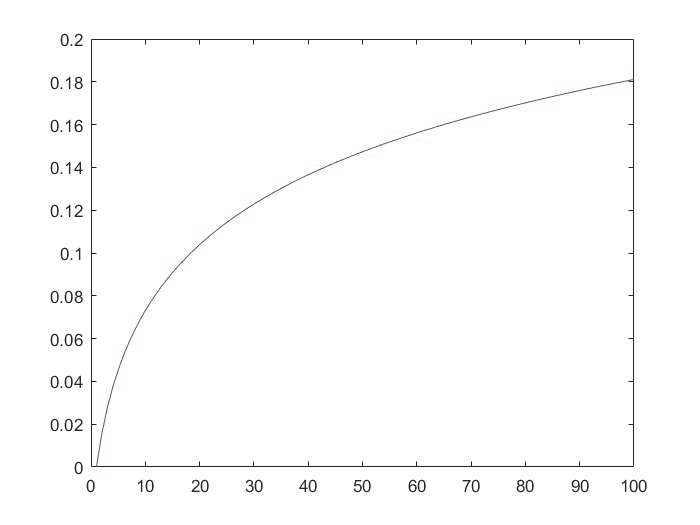
\includegraphics[height=8cm]{images/exchange-discount.png}

\caption{$LRC$ token deposit rank and cost for discount}
\label{fig:discount}

\end{figurehere}
\end{center}


\subsection{Fraud and Attack Protection}

\subsubsection{Exchange Covered Interest Arbitrage}

Loopring endeavors to create a fair ecosystem and to find a balance between customers (users) and exchanges. First, we will explain how an exchange could achieve a zero-risk covered interest arbitrage.

Assume there are two orders $O_{a\rightarrow b}$, $O_{b\rightarrow a}$ that form a loop, $r_{a\rightarrow b} \cdot r_{b\rightarrow a} > 1$. An exchange can input three new orders between those two. $O_{b\rightarrow c}$, $O_{c\rightarrow d}$, $O_{d\rightarrow b}$, to create a five order loop,  $r_{a\rightarrow b} \cdot r_{b\rightarrow c} \cdot r_{c\rightarrow d}\cdot r_{d\rightarrow b}\cdot r_{b\rightarrow a} = 1$. An exchange could bring the possible cost down to zero once the transaction completed, implementing zero-risk covered interest arbitrage, $O_{b\rightarrow c}\rightarrow O_{c\rightarrow d}\rightarrow O_{d\rightarrow b}$. In order to stop these parameters, Loopring requires: {\bfseries a verified loop that cannot create a further sub-loop to continue trading}.

\subsubsection{Denial-of-Service}

Loopring allows exchanges to selectively handle orders. An exchange can set up their own criteria and may choose to hide or reveal these criteria. Therefore Loopring does not see denial of service as a form of unethical behavior.

\subsubsection{Massive Tiny Order Attacks}
A user can send out a large amount of tiny orders to attack exchanges. Exchanges however, will reject most of these tiny orders because they do not yield satisfying profit when matched. As denial-of-service is not deemed as a form of attack, massive tiny order attacks are not feasible.

\subsubsection{Insufficient Balance}

Malicious users may sign and spread out orders in which the order value is not zero,but the wallet address actually has a zero balance. This again is a not a good way to attack exchanges. Exchanges will monitor and notice that some orders' actual balance is zero and update these orders states accordingly, then discard them.  

Exchanges do have to spend time to update the order status, but can also choose to minimize these effort by, for example, blacklisting some addresses and drop all related orders.

\subsubsection{Ring Filch}

A deviant exchange could monitor all unconfirmed Match-Rings and broadcast the same rings with their own digital signature. We call this Ring Filch. In order to prevent Ring Filch Loopring requires exchanges to use two steps in order to submit the order: 
\begin{itemize}
  \item Submit the hash of a Match-Ring, then wait for confirmation.
  \item Submit the ring itself.
\end{itemize}
Hash rate:
$$h = H(r,  nonce)\text{, }$$
where $H()$ is a one-way hash function, $r$ is Match-Ring record. Hash function contains a random number $nonce$.

\subsection{Market Depth\label{sec: marketdepth}}

Exchanges do not need to offer market depth data. Under this ecosystem, it is possible for both single entities and corporations to possibly pool all unclosed orders into one instance of market depth data. We can ascertain trading data between any two ERC20 tokens according to the agreement in chapter 3.3.

\subsection{Data Structure\label{sec: dataformat}}

All orders can be represented by using one data structure due to adopting the OTC module. This data structure contains both a digital signature and all parameters. Before the signature, the parameter data is connected from the orders into a set of data, the order's hash is calculated by using Keccak SHA3 method, and then signed by using this account's private keys with ECDSA.


\begin{verbatim}
message Order {
 address protocol;
 address owner;
 address outToken;
 address inToken;
 uint256 outAmount;
 uint256 inAmount;
 unit256 expiration
 unit256 fee;
 uint8 marginSplit;
 unit8 v;
 bytes32 r;
 bytes32 s;
}
\end{verbatim}

Though there is no indicated price from the order, we are still able to find out through the formula: $outAmount / inAmount$ to determine the exchange rate $r$. The actual exchange rate must be less than $r$. A user-friendly exchange should allow user to input $outAmount$, $inAmount$, selling and asking price, and use any two of those numbers in order to calculate the missing $outAmount$ or $inAmount$ figure.
Actual orders can be defined in two different ways: Definition A - transaction can be completed once the number of tokens sold reaches $outAmount$ ; Definition B - transaction can be completed once the number of tokens purchased reaches $inAmount$; Therefore, we can setup a quote for exchange and mix-matching contract to help to define the trade. At our initial version, we would support Definition A only.

The exchange can create a Match-Ring by using this data structure:
\begin{verbatim}
rmessage MatchRing {
  Order[] orders;
  address feeRecipient;
  unit256 additionalDiscount;
  unit256 nonce;
  unit8 v;
  bytes32 r;
  bytes32 s;
}
\end{verbatim}


\subsection{Order Status\label{sec: orderstate}}


An order cannot be modified once it has been signed and announced. Data will be updated on the blockchain once the smart contract finds the matched order. Thus $inAmount$ and $outAmount$ will be modified correspondingly with the updated price. If $inAmount / outAmount$ shows 0,  it means that the order has been fully closed. For example, if the user wants to cancel the order, a special request will be filed,  $inAmount / outAmount$ will be 0 to close the order. An expired order will not be updated on the blockchain - it can be tracked through the final cutting time. Therefore, we expect most of the orders will expire or be invalidated.

\subsection{Smart Contracts\label{sec: contracts}}

Loopring consists of many smart contracts, including:

\begin{itemize}
 \item \textbf{Mix-Matched Contract} is responsible for ensuring each order status in the loop, calculating the price and volume,  transferring and interaction with other smart contracts, API for Loopring;
 \item  \textbf{Order Contract} updates order database and supports cancelling policy;
 \item \textbf{Registration Contract} maintains and upgrades service for exchanges who accepted Loopring, support the token deposit from exchange and defaulted parameters backup;
 \item \textbf{Stats Contract} calculates the exchange volume and price between two tokens.

\end{itemize}

\begin{comment}
\subsection{支持ENS\label{sec: registration}}

\end{comment}

\section{Protocol Token \label{sec: protocoltoken}}


We will issue a token based on ERC20 Ethereum Token Standard called $LRC$ (displays in italics).


\subsection{Token Application}

$LRC$ will be used in the following areas:

\begin{itemize}
 \item \textbf{Gas Fees} --- $LRC$ can be paid as transaction fees to the exchange. It will be simple and productive for the exchange to calculate all the cost in $LRC$. Same as request sender and receiver. We mentioned this fee structure in chapter\ref{sec: fee}.
 \item \textbf{Deposit for Exchange Registration} --- The decentralized exchange mechanism has no limits on location or time. Consequently, exchanges with a high turnover would receive more orders and get more users. As a result, we have designed a policy for such exchanges that allow users to use $LRC$ to deposit into a smart contract in order to increase the exchanges credibility. Moreover, it can also protect users from certain adverse circumstances.
\end{itemize}

\subsection{Decentralized Governance}
Regulation has been updated as well as the exchanges mechanism. Any $LRC$ holders have the voting power $S$, and number of the pledging $N$ and pledging time $CoinAge$
$$S = f(N,  CoinAge)\text{, }$$
where $CoinAge = H_{c}-H_{s}$. Joining CoinAge aids to protect customers from speculation.

The decentralized mechanism includes token registration, exchange registration, stat hash, deposit scale, maximum length, discount hash, and subcontract address.
 \begin{itemize}
   \item \textbf{Token registration} Loopring would adjust token; low trading volume will be eliminated and new popular token will be replaced. All the adjustments have to be recorded on the smart contract.
  \item \textbf{Exchange registration} Only those exchanges that accept Loopring would allow trading to begin.
   \item \textbf{Stat hash} Data will increase to a certain amount after a long period of operation. The more data exchanges have, the more accurate the system computation ability will be.
  \item \textbf{Deposit scale} Deposit for each exchange should be measurable. If the amount is large, the liquidation gets worse; and vice verse.
   \item \textbf{Maximum length} Technically, more orders can create more profit, however the risk of failure also increases, as well as the trading cost.
   \item \textbf{Discount hash} Discount hash will be adjusted with the market. The below figure shows the normal market (represented by the blue line), the supply market (represented by the blue line), and the demand market (represented by the red line ).
\begin{center}
\begin{figurehere}
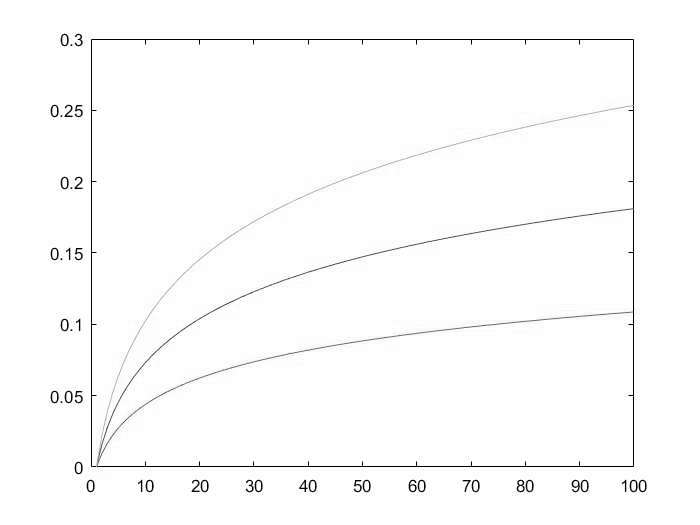
\includegraphics[height=10cm]{images/rate_adjust.jpg}
\caption{discount rate after adjustment}
\label{fig: dischargeRateAdjust}
\end{figurehere}
\end{center}

   \item \textbf{Subcontract address} If Loopring exchange is based on the Ethereum ecosystem, then the smart contract cannot be modified. Therefore, the users must update Loopring's subcontract in order to modify the subcontract address.
 \end{itemize}

%\footnotemark

\subsection{Token's Liquidity}

Loopring's token is based on the ERC20 Ethereum Token Standard and can be liquidated through a Loopring smart contract. This means that LRC trading can be done through a centralized exchange. All the ERC20 Ethereum tokens can be exchanged to LRC token (assume pre-order is LRC, with zero fee) by adopting Loopring's decentralized mechanism.


\section{Exchange\label{sec: exchange}}

An exchange is unable to guarantee that all transactions will lead to profits after Loopring adoption. The first reason is high operation cost. Secondly, high expectation may not result in projected outcomes. There are few other reasons that would cause this saturation. Overall,  both the exchange platform and other parties have a reciprocal relationship: the exchange looks for a profitable order, while order senders look for an exchange with the lowest fee.
An exchange is not responsible for users ERC20 token after accepting Loopring. The workload has moved from money deposit, withdrawal,  and internal virtual account management services, to mix-matched order service. Meanwhile, for the users, Loopring does not require the customer to deposit or lock any asset, meaning an asset has zero third-party custod risk. Concurrently, a single order can mix and match multiple trades. For Non-ERC20 assets, an exchange can offer an asset tokenization service.

\subsection{Regular and Loopring Exchange Comparison}
In a regular exchange, the "Maker" sends an order, and the "Taker" receives this order. The exchange's price highly depends on the sender's end. However Loopring has adopted the over-the-counter (OTC) model.
In the current marketplace, centralized exchanges pose considerably high risk for users trading in these platforms; there are no laws to regulate the exchange if they vanish. But with Loopring, users do not deposit money to centralized exchange. All of the transactions will be made through the user's coin address.
Loopring also changes the "Trading Pair" concept utilized by centralized exchanges. Transactions can be completed with multiple parties, rather than two parties in current exchange scenarios.


\begin{table}[hbt]
  \centering
\begin{tabular}{p{5cm}|p{2.5cm}|p{2.5cm}} %设置了每一列的宽度,强制转换。
&Centralized Exchange & Loopring Exchange \\ %用&来分隔单元格的内容 \\表示进入下一行
    \hline
Deposit for the order& Yes & No \tablefootnote{Exchanges execute under Loopring ecosystem do not require any deposit - Tokens are kept in user's wallet, no transaction will be made before the full contract close. As a result, no account can be stolen, or asset lost risk.}\\
\hline
Frozen Account& Yes & No \tablefootnote{Loopring exchanges do not require freeze trading fund --- If a user partially or fully modifies the fund, the contract will be withdraw automatically.}\\
\hline
Deposit/Withdraw& Yes & No \tablefootnote{The sender's order can be distributed to multiple receivers to be partially or fully fulfilled under Loopring ecosystem.}\\
\hline

Internal Trading Risk& Yes & No\tablefootnote{All matching trades are based on smart contract on blockchain, data are immutable and transparent.}\\
\hline
Customer loss from exchange closing& Yes & No\tablefootnote{ Loopring exchanges are not responsible for tokenization, thus Loopring users will not be affected if an exchange becomes insolvent. For example, a blockchain account will not affected if mining is terminated. In conclusion, exchanges are responsible for matching trades. Loopring's smart contract will complete clearing and settlement, furthermore, assets are always kept in user's blockchain account.}\\
\hline
Transaction is the main income& Yes & No\tablefootnote{Transaction fee is not a mainstream income for Loopring exchanges, mainstream comes from “profit of transaction margin”, because it can effectively encourage trade matching.}\\
\hline
Accept Fiat Money& Yes & Yes\tablefootnote{Loopring exchanges fully support asset tokenization, hence, it requires legitimate currency being tokenized on ERC20 standard.}\\
\hline
Can be traded among multiple exchanges& No & Yes \tablefootnote{Loopring allows multiple Loopring exchanges to partially or fully trade off one order at same time.}\\
\hline
Fairness for Maker and Taker& No & Yes \tablefootnote{Transaction price is closed to the balance price instead of being tendered to the maker's offer price under Loopring protocol.}\\
\hline
Mix and Match Trading& No & Yes\tablefootnote{ Loopring exchanges' multiple supporting feature can help sender to find the most profitable order.}\\
\hline
Supervision & Strong & Weak\tablefootnote{Loopring exchanges do not require a deposit. Clearing and settlement are made through the open source smart contract. Therefore, regulation is not necessary if there is no asset tokenization occurrence.}\\

  \end{tabular}

\caption{Contrast between a centralized exchange and Loopring exchange} %显示表格的标题
\end{table}

%\footnotemark


\section{Summary\label{sec: summary}}

Loopring is a protocol that facilitates decentralized exchange of ERC20 tokens on the Ethereum blockchain. Loopring allows multi-token transaction exchange, as well as liquidation exchange on the blockchain under different circumstances. Loopring offers benefits to both users and exchanges by deferring risk from both parties in decentralized smart contracts, minimizing fees and cost to create more profitable orders through ring-matching and order-sharing, and as a cross-platform protocol. Loopring protocol fits any ERC20 and smart contract blockchain platform. After many discussions,  our team will develop Loopring on the Ethereum blockchain.

\section{Acknowledgements\label{sec: acknowledgement}}

We would like to express our gratitude to our mentors, advisers and to the many people in the community that have been so welcoming and generous with their knowledge. In particular, we would like to thank Shuo Bai (from ChinaLedger); Professor Haibin Kan; Alex Cheng, Hongfei Da; Yin Cao; Xiaochuan Wu; Zhen Wang, Wei Yu, Nian Duan, Jun Xiao, Jiang Qian, Jiangxu Xiang, Yipeng Guo, Dahai Li, Kelvin Long, Huaxia Xia, Jun Ma, and Encephalo Path for reviewing and providing feedback on this project. We also welcome more feedback from the community.

\newpage  
\bibliography{whitepaper}
\bibliographystyle{unsrt}

%\newpage
%
%\begin{appendices}
%\section{$LRC$ Token Crowdsale\label{sec: ico}}
%
%We plan to issue 100 million LRC token, 80 million tokens will be allocated to crowdsale participators, and the remaining 20 million tokens will be allocated to the foundation initiator for maintenance and development of the Loopring community over the next 5 years.
%
%ICO will start pre-sale to investors and crowdsale in 2017 July. We plan to raise XXXX ETH
%Initial spending plan;
%
%\begin{table}[hbt]
% \centering
% \begin{tabular}{l|c}
%   Purpose    & Percentage\\
%  \hline
% Tech Development  & 50\% \\
% Community Building & 20\% \\
% Marketing     & 15\% \\
% Legal and Law   & 15\% \\
% \end{tabular}
% \caption{ Plan for token expense}
%\end{table}
%
%
%
%Project ICO and Timetable
%\begin{table}[hbt]
% \centering
% \begin{tabular}{l|l}
%Time  & Target\\
%  \hline
% 2017/06 & Whitepaper release, Project start-off \\
% 2017/07 & Module Development Completion \\
% 2017/08 & Loopring open source committee(Foundation)set and Pre ICO closed \\
% 2017/08 & ICO schedule \\
% 2017/09 & ICO start \\
% 2017/10 & ICO close and release result \\
% 2017/11 & $LRC$Token IOU launch at exchange \\
% 2017/12 & Test $LRC$ token on ETH \\
% 2018/02 & Commencement \\
% 2018/04 & Issue $LRC$ token on ETC \\
% \end{tabular}
% \caption{Project Schedule}
%\end{table}
%
%\subsection{ETH/ETC Due-chain issue\label{sec: chains}}
%
%Alhough we only accept ETH as our ICO token, we also consider ETC token's potential on developing smart contract. Hence, we will issue our token $LRC$ on both Ethereum (ETH)and Ethereum Classic(ETC).
%
%
%\subsection{Risk Awareness\label{sec: risks}}
%
%Initial crypto-token offering (ICO) is a popular way for crowdsale, however it contains certain risks. Participators should be fully aware of all the potential risk and The Loopring Foundation hereby expressly disclaims its liability, and shall in no case be liable to any person, for: 
%\begin{itemize}
% \item any person's participation in the Campaign in violation of any anti-money laundering, counter-terrorism financing or other regulatory requirements that are imposed in any jurisdiction;
% \item any person's participation in the Campaign in violation of any representation, warranty, obligation, covenant or other provision under this prospectus, and the resulting failure or inability to retrieve his/her payment or to claim relevant purchased $LRC$ for Crowdsale;
% \item early termination of the Campaign for any reason;
% \item failure or abortion of the Quantum development and resulting failure to deliver the purchased $LRC$ for Crowdsale to the Purchasers;
% \item any risk factors disclosed in this Prospectus and any damage, loss, claim, liability, punishment, cost or other adverse impact that is caused by, associated with, in connection with, incidental to or consequential to that risk factor.
% \item if there is any separate agreement between a Purchaser and a Crowdsale Intermediary, this Prospectus shall take precedence over that agreement in all respects. The Loopring Foundation shall in no case be bound by, and hereby disclaims any liability under, the foregoing agreement.;
% \item failure or abortion of the Loopring development and resulting failure to deliver the purchased $LRC$ for crowdsale to the Purchasers;
%
%\end{itemize}
%
%
%
%\end{appendices}
\end{document}
